\chapter{DC Circuit Analysis}

In the most basic circuit, you have only a battery and a resistor:
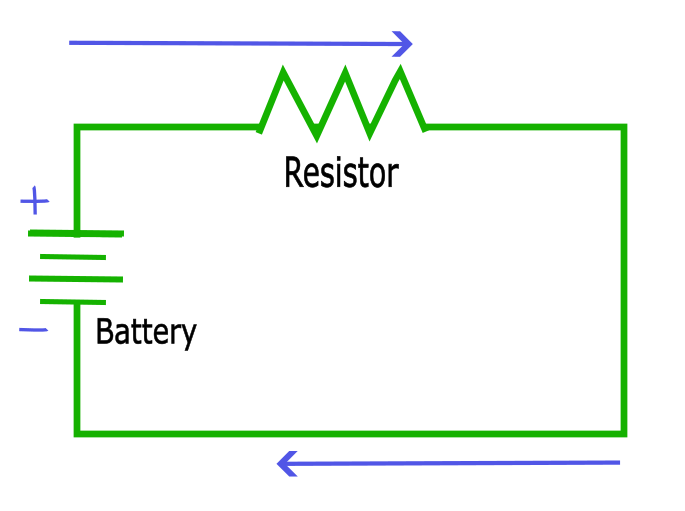
\includegraphics[width=0.8\textwidth]{DC_Circuit_Diagram.png}

\begin{circuitikz}
\draw (0,0) to[battery1,invert,l=$6V$] ++(0,3)
to ++(3,0)
to [R=$3\Omega$, /tikz/circuitikz/bipoles/length=1.0cm,i=2A] ++(0,-3) -- (0,0);
\end{circuitikz}

In this case, you only need Ohm's Law: $V = I R$.  In this case, $6V = 3\Omega \times 2A$.
% ADD: Define Ohm's Law
\begin{Exercise}[title={Ohm's Law}, label=ohms_check]

  How many amps are going around the circuit?
  
  \vspace{1cm}

\begin{circuitikz}
\draw (0,0) to[battery1,invert,l=$24V$] ++(0,3)
to ++(3,0)
to [R=$6\Omega$, /tikz/circuitikz/bipoles/length=1.0cm,i={? A}] ++(0,-3) -- (0,0);
\end{circuitikz}

  
\end{Exercise}
\begin{Answer}[ref=ohms_check]

  $V = I R$ so $I = \frac{V}{R} = \frac{24V}{6\Omega} = 4A$.
  
\end{Answer}
% KA: https://youtu.be/F_vLWkkOETI

\section{Resistors in Series}

When you have two resistors wired together in a long line, we say they
are ``in series''.  If you have two resistors $R_1$ and $R_2$ wired in
series, the total resistance is $R_1 + R_2$.

In this diagram, for example, the total resistance is $5\Omega$.

\begin{circuitikz}
\draw (0,0) to[battery1,invert,l=$10V$] ++(0,5)
to ++(3,0)
to [R=$3\Omega$] ++(0,-2.5)
to [R=$2\Omega$] ++(0,-2.5) -- (0,0);
\end{circuitikz}

The current flowing through the circuit, then, is $10/4 = 2A$.

By Ohm's law, the voltage drop across the upper resistor is $I R = 2A \times 3\Omega = 6V$.

The voltage drop across the lower resistor is $I R = 2A \times 2\Omega = 4V$.

Notice that the battery pumps the voltage up to $10V$, then the two
resistors drop it by exactly $10V$. This is known as ``Kirchhoff's
Voltage Law'':
% KA: https://youtu.be/4rsswT_Rv1M

\begin{mdframed}[style=important, frametitle={Kirchhoff's Voltage Law}]\index{Kirchhoff's voltage law}
As you make a loop around a circuit, the sum of the voltage increase
must equal the sum of the voltage decrease.
\end{mdframed}

The negative end of the battery as connected to ``ground'' (
it has zero voltage), then we can draw a diagram with the
voltages(That symbol in the lower right represents a connection to ground).

\begin{circuitikz}
\draw (0,0) to[battery1,invert,l=$6V$] ++(0,5) 
to [-*] ++(3,0) node[anchor=west] {10V}
to [R=$3\Omega$,-*] ++(0,-2.5) node[anchor=west] {4V}
to [R=$2\Omega$,-*] ++(0,-2.5) node[anchor=west]{0V} node[ground]{} --(0,0);
\end{circuitikz}


\begin{Exercise}[title={Resistors In Series}, label=series_resistor]

  What is the current going around the circuit?
  
  What is the voltage drop across each resistor?
  
  \vspace{1cm}
\begin{circuitikz}
\draw (0,0) to[battery1,invert,l=$16V$] ++(0,5) 
to [-*] ++(3,0) node[anchor=west] {16V}
to [R=$5\Omega$,-*] ++(0,-2.5) node[anchor=west] {?}
to [R=$3\Omega$,-*] ++(0,-2.5) node[anchor=west]{0V} node[ground]{} --(0,0);
\end{circuitikz}


\end{Exercise}
\begin{Answer}[ref=series_resistors]

  There is a total resistance of $8\Omega$, so your 16V will push 2A
  of current around the circuit.

  2A going through a $5\Omega$ resistor represents a 10V drop.

  2A going through a $3\Omega$ resitor represents a 6V drop.
  
\end{Answer}


\section{Resistors in Parallel}

Look at this circuit. Note that the current can go two different paths.

\begin{circuitikz}
\draw (0,0) to[battery1,invert,l=$12V$] ++(0,3)
to ++(3,0)
to [R=$2\Omega$, /tikz/circuitikz/bipoles/length=1.0cm] ++(0,-3) -- (0,0);
\draw (3,3) -- (5,3)
to [R=$3\Omega$, /tikz/circuitikz/bipoles/length=1.0cm] ++(0,-3) -- (3,0);
\end{circuitikz}

There is 12 volts pushing current through both resistors. So 6A will
go through the 2$\Omega$ resistor and 4A will go through the 3$\Omega$
resistor.

\begin{circuitikz}
\draw (0,0) to[battery1,invert,l=$12V$] ++(0,3)
to ++(3,0)
to [R=$2\Omega$, /tikz/circuitikz/bipoles/length=1.0cm,i=6A] ++(0,-3) -- (0,0);
\draw (3,3) -- (5,3)
to [R=$3\Omega$, /tikz/circuitikz/bipoles/length=1.0cm,i=4A] ++(0,-3) -- (3,0);
\end{circuitikz}

Thus, a total of 10 A will be going through the battery.

Imagine you are a battery. You can't see that you have two resistors.
What does it feel like to you? $\frac{V}{I} = R$, and $V= 12$ and $I =
10$.  So the effective resistance of the two resistors in parallel is
$\frac{12}{10}$ or $\frac{6}{5} \Omega$.

\begin{mdframed}[style=important, frametitle={Resistance in Parallel}]\index{resistance!in parallel}
If you have several resistances $R_1, R_2, \ldots, R_n$ wired in
parallel, their effective resistance $R_t$ is given by

$$\frac{1}{R_t} = \frac{1}{R_1} + \frac{1}{R_2} + \ldots + \frac{1}{R_n}$$

\end{mdframed}

In our example:

$$\frac{1}{R_t} = \frac{1}{2} + \frac{1}{3} = \frac{5}{6}$$

Thus $R_t =  \frac{6}{5}\Omega$.

\begin{Exercise}[title={Resistors In Parallel}, label=parallel_resistors]

  What is the current going through the battery?
  What is the drop over the $4\Omega$ resistor?
  What is the current in each branch?

  \vspace{1cm}

  \begin{circuitikz}
\draw (0,0) to[battery1,invert,l=$12V$] ++(0,3)
to [R=$4\Omega$, /tikz/circuitikz/bipoles/length=1.0cm] ++(3,0) node [yshift=0.3cm] {? V}
to [R=$6\Omega$, /tikz/circuitikz/bipoles/length=1.0cm,i={? A}] ++(0,-3) node[ground]{} -- (0,0);
\draw (3,3) -- (5,3)
to [R=$3\Omega$, /tikz/circuitikz/bipoles/length=1.0cm,i={? A}] ++(0,-3) -- (3,0);
\end{circuitikz}

\end{Exercise}
\begin{Answer}[ref=parallel_resistors]
  The effective resistance of the $6\Omega$ and the $3\Omega$ is $2\Omega$ because 

  $$\frac{1}{R_T} = \frac{1}{6} + \frac{1}{3} == \frac{1}{2}$$

  So the battery experiences a resistance of $4\Omega + 2\Omega =
  6\Omega$.  A $12V$ will push 2A through a resistance of $6\Omega$.

  The voltage drop across the $4\Omega$ resistor is $2A \times 4\Omega
  = 8V$. Thus there will be a 4V drop across the two resistors in
  parallel.  So 2/3 A will flow through the $6\Omega$ resistor. 4/3 A
  will flow through the $3\Omega$ resistor.

    \begin{circuitikz}
\draw (0,0) to[battery1,invert,l=$12V$] ++(0,3)
to [R=$4\Omega$, /tikz/circuitikz/bipoles/length=1.0cm] ++(3,0) node [yshift=0.3cm] {8 V}
to [R=$6\Omega$, /tikz/circuitikz/bipoles/length=1.0cm,i={2/3 A}] ++(0,-3) node[ground]{}-- (0,0);
\draw (3,3) -- (5,3)
to [R=$3\Omega$, /tikz/circuitikz/bipoles/length=1.0cm,i={4/3 A}] ++(0,-3) -- (3,0);
\end{circuitikz}
  
\end{Answer}

\section{Cognitive bias: Survivorship bias}

You will pay more attention to those that survived a process than
those who failed.

After looking at a lot of old houses, you might say ``In the 1880s,
they built great houses.'' However, you haven't seen the houses that
were built in the 1880s and didn't survive.  Which houses tended to
survive for a long time? Only the great houses -- you are
basing your opinion on a very skewed sample.

